\vspace{-2mm}
\section{Unified Hand Action Space}
\vspace{-2mm}
\label{sec:method}
% Our method is inspired by the RobotFingerPrint (RFP) intermediate grasp representation~\cite{khargonkar2024robotfingerprint} for robotic grasp synthesis. In RFP, the interior palm surfaces of multiple robotic grippers are mapped using a ``maximal sphere'' representation. Specifically, each point on the gripper's palm interior is assigned spherical coordinates $  (\lambda, \phi)  $, thereby establishing a direct correspondence to a point on the surface of the unit sphere $  S  $, i.e., every palm surface point $  p_{\text{surface}}  $ satisfies $  p_{\text{surface}} \in S  $.

% This mapping is applied to a grasp dataset to train a Conditional Variational Autoencoder (CVAE) generative neural network. The CVAE learns to predict unified gripper coordinates for the surface points of objects, producing maps in which each predicted point corresponds directly to a point on the gripper palm via the shared sphere representation. These predicted maps are subsequently employed in an optimization algorithm to derive a joint configuration $  \mathbf{q}_G  $ of each gripper.


The Unified Hand Action Space (UHAS) is motivated by the central question of whether robotic hand control can be expressed through geometric deformations of a canonical sphere surface. A sphere provides a natural unified representation because it defines a continuous, closed, and topology-agnostic surface that can be consistently parameterized across robotic hands with different kinematic structures and numbers of fingers. Moreover, many grasping and dexterous manipulation behaviors can be interpreted as coordinated radial and angular interactions around an object-centered workspace, making the sphere a convenient geometric abstraction for hand control.


% The Unified Hand Action Space (UHAS) is motivated by the central question of whether robotic hand control can be expressed through geometric deformations of a canonical sphere surface. 


% Building upon the unified hand representations introduced in~\cite{khargonkar2024robotfingerprint}, which normalize diverse robotic hands into a shared representation for grasp synthesis, we propose to directly use the canonical sphere surface as a unified action space for hand control. Specifically, by binding the fingers of a robotic hand to corresponding points on the sphere surface, variations in the hand joint configuration $ \mathbf{q}_H $ can be represented as deformations or displacements of the sphere surface points $ \mathcal{P}_S $, as illustrated in Figure~\ref{fig:motivation}. This formulation transforms embodiment-specific joint control into a shared geometric manipulation problem, enabling a learned policy to generate dexterous behaviors across multiple robotic hand embodiments by operating directly in the unified spherical domain.



% In this paper, we propose a method that leverages these sphere representations for the following reason: variations in the gripper's joint configuration $  \mathbf{q}_G  $ can be represented as deformations (or displacements) of the corresponding points of the sphere surface. This relationship is illustrated in Figure~\ref{fig:motivation}.

% \begin{figure}[t]
%     \centering
%     \begin{center} 
%         \includegraphics[width=\linewidth]{figures/Gripper_sphere_Correspondence_v2.pdf}
%         \caption{Hand--sphere point-wise correspondence in the Unified Hand Action Space (UHAS). 
%     The rainbow coloring encodes the direct mapping between locations on the sphere surface \(\mathcal{P}_S\) and the corresponding contact points on the gripper's palm and fingers. 
%     \textbf{Left}: reference gripper configuration \(\mathbf{q}_{G_{S^*}}\) while grasping a perfect sphere. 
%     \textbf{Right}: example gripper configurations corresponding to different sphere surface point arrangements.} 
%     \label{fig:motivation}
%         \label{fig:motivation}
%     \end{center}
%     \vspace{-4mm}
% \end{figure}

\begin{figure}[h]
    \centering
    \begin{center} 
        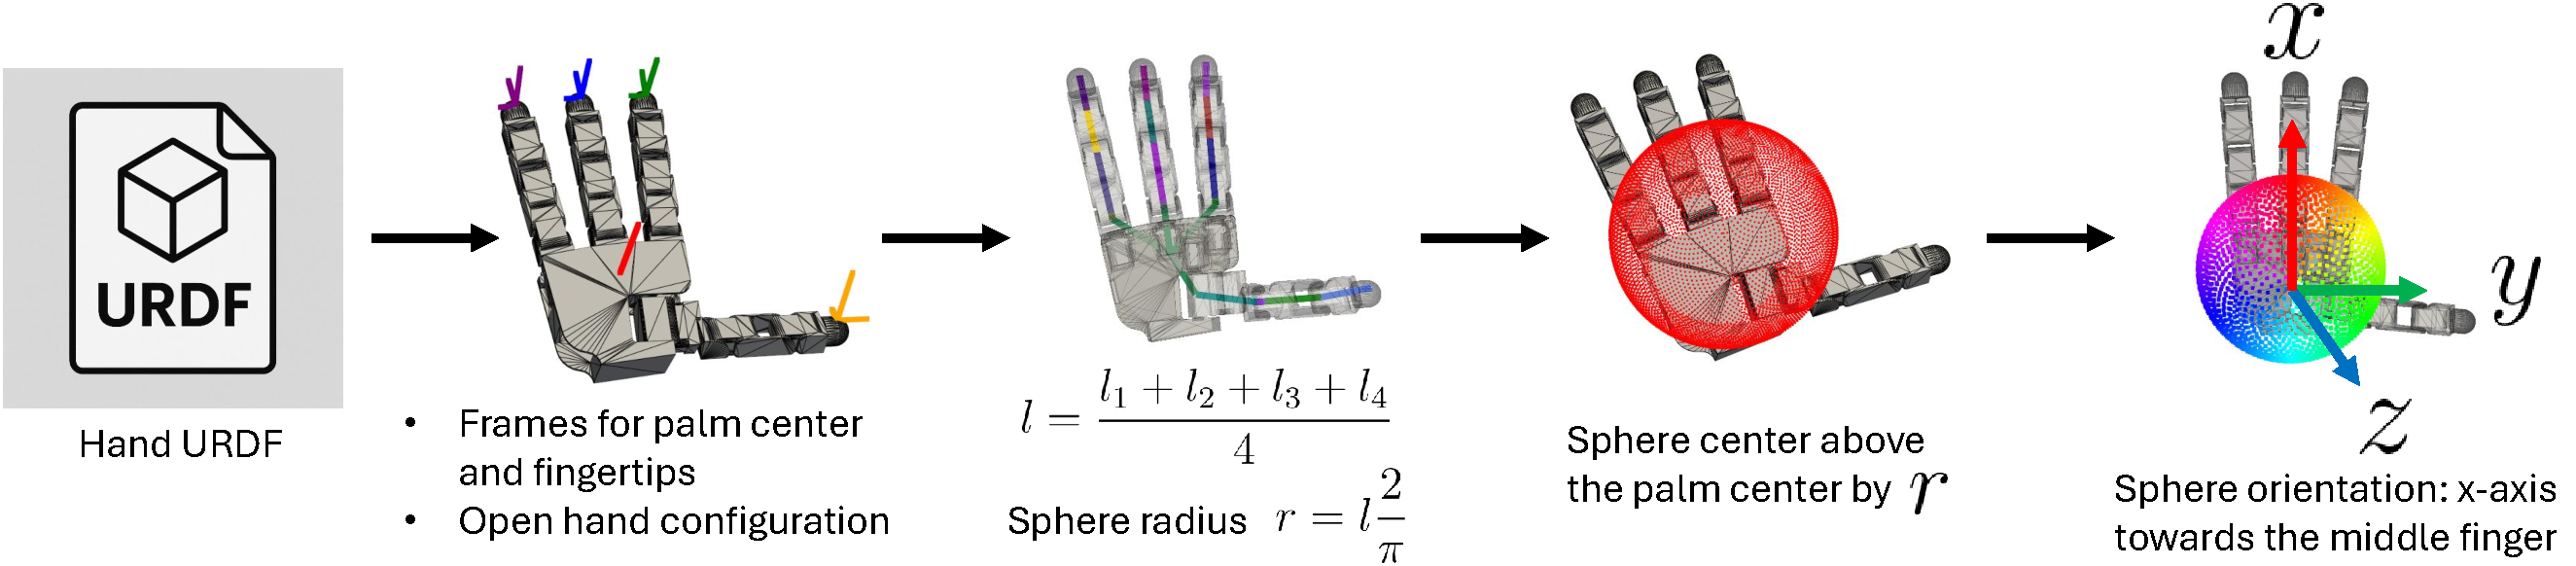
\includegraphics[width=\linewidth]{figures/sphere_creation.pdf}
        \caption{Illustration of the process of creating a sphere for a robotic hand given its URDF.}
    \label{fig:sphere_construction}
    \end{center}
    \vspace{-6mm}
\end{figure}

\subsection{Automatic Sphere Creation for a Robotic Hand}
\label{sec:construction}

Given a robotic hand URDF model, we automatically construct the canonical sphere through kinematic analysis and geometric normalization, as illustrated in Fig.~\ref{fig:sphere_construction}. We first identify the palm and fingertip coordinate frames in an open-hand configuration, where the fingers are fully extended and the fingertip normals approximately align with the palm normal. We then compute the palm center by averaging the finger root positions and measure the average distance $l$ from the palm center to the fingertips. The sphere radius is defined as $r=\frac{2l}{\pi}$, placing the sphere within the natural grasping workspace of the hand and approximately covering a $90^\circ$ arc from the palm center to the fingertips.

Next, the sphere center is positioned along the outward palm normal at a distance $r$ from the palm center, placing the sphere within the natural grasping workspace of the hand where the fingers tend to converge during grasping and dexterous manipulation. To obtain a canonical orientation shared across embodiments, the sphere coordinate frame is defined such that its positive $z$-axis aligns with the outward palm normal and its positive $x$-axis aligns with the middle finger direction. The $y$-axis is then uniquely determined by the resulting $xz$-plane according to the right-hand rule.

To remove embodiment-specific scale differences, all distances in the sphere coordinate frame are normalized by the hand-specific radius $r$. This normalization maps the canonical sphere to a \emph{unit sphere}, producing a scale-invariant representation shared across robotic hands with different kinematic structures and numbers of fingers. The resulting normalized sphere coordinate system defines the Unified Hand Action Space (UHAS), enabling a unified geometric action representation for cross-embodiment policy learning and transfer. Although the UHAS operates on a normalized unit sphere, the corresponding hand-specific sphere parameters are preserved and later used by the Cascade Inverse Kinematics (CIK) algorithm to recover embodiment-specific hand configurations.




% We construct the UHAS by performing a kinematic analysis of each hand. The  analysis is based on the gripper's kinematic tree, local fingertip coordinate frames, and a palm coordinate frame. 

% In each fingertip frame, the $  z  $-axis is aligned with the outward normal of the fingertip's contact surface (i.e., the direction perpendicular to the surface and pointing away from the fingertip material), while the $  x  $-axis points along the longitudinal direction of the finger (i.e., the direction the finger is pointing). The palm frame has its $  z  $-axis aligned with the outward-pointing palm normal. 

% Additionally, an initial open joint configuration $  \mathbf{q}_{G_0}  $ is used, in which the fingers are fully opened such that the $  z  $-axes of the fingertip frames are aligned as closely as possible to the palm normal.

% To construct the sphere coordinate frame, we first compute the palm center $  \mathbf{c}_p  $ as the geometric centroid of the finger root positions, obtained from their $  xy  $-coordinates expressed in the palm frame. The palm frame origin is then translated to this palm center.
% The sphere radius $  r  $ is determined by computing the Euclidean distances from $  \mathbf{c}_p  $ to each fingertip in the initial open configuration $  \mathbf{q}_{G_0}  $. These distances are averaged to obtain $  d_{\text{avg}}  $. The radius is then set to $r = \frac{d_{\text{avg}}}{\pi/2}.$
% The transformation from the (translated) palm frame to the sphere frame consists of a translation of distance $  r  $ along the positive $  z  $-axis followed by a $  180^\circ  $ rotation about the $  x  $-axis.

% For additional normalization and canonical alignment across different grippers, we identify the ``middle finger'' by computing the azimuthal angles $  \theta  $ of all finger roots in the preliminary sphere frame. The middle finger is selected as the one whose root angle is closest to the circular mean of these angles. The positive $  x  $-axis of the final sphere frame is then aligned with the kinematic chain of this middle finger, such that both its root and its fingertip lie on the $  xz  $-plane of the sphere frame.
% This construction is illustrated in Figure~\ref{fig:sphere_construction}.

\begin{figure}[h]
    \centering
    \begin{center} 
        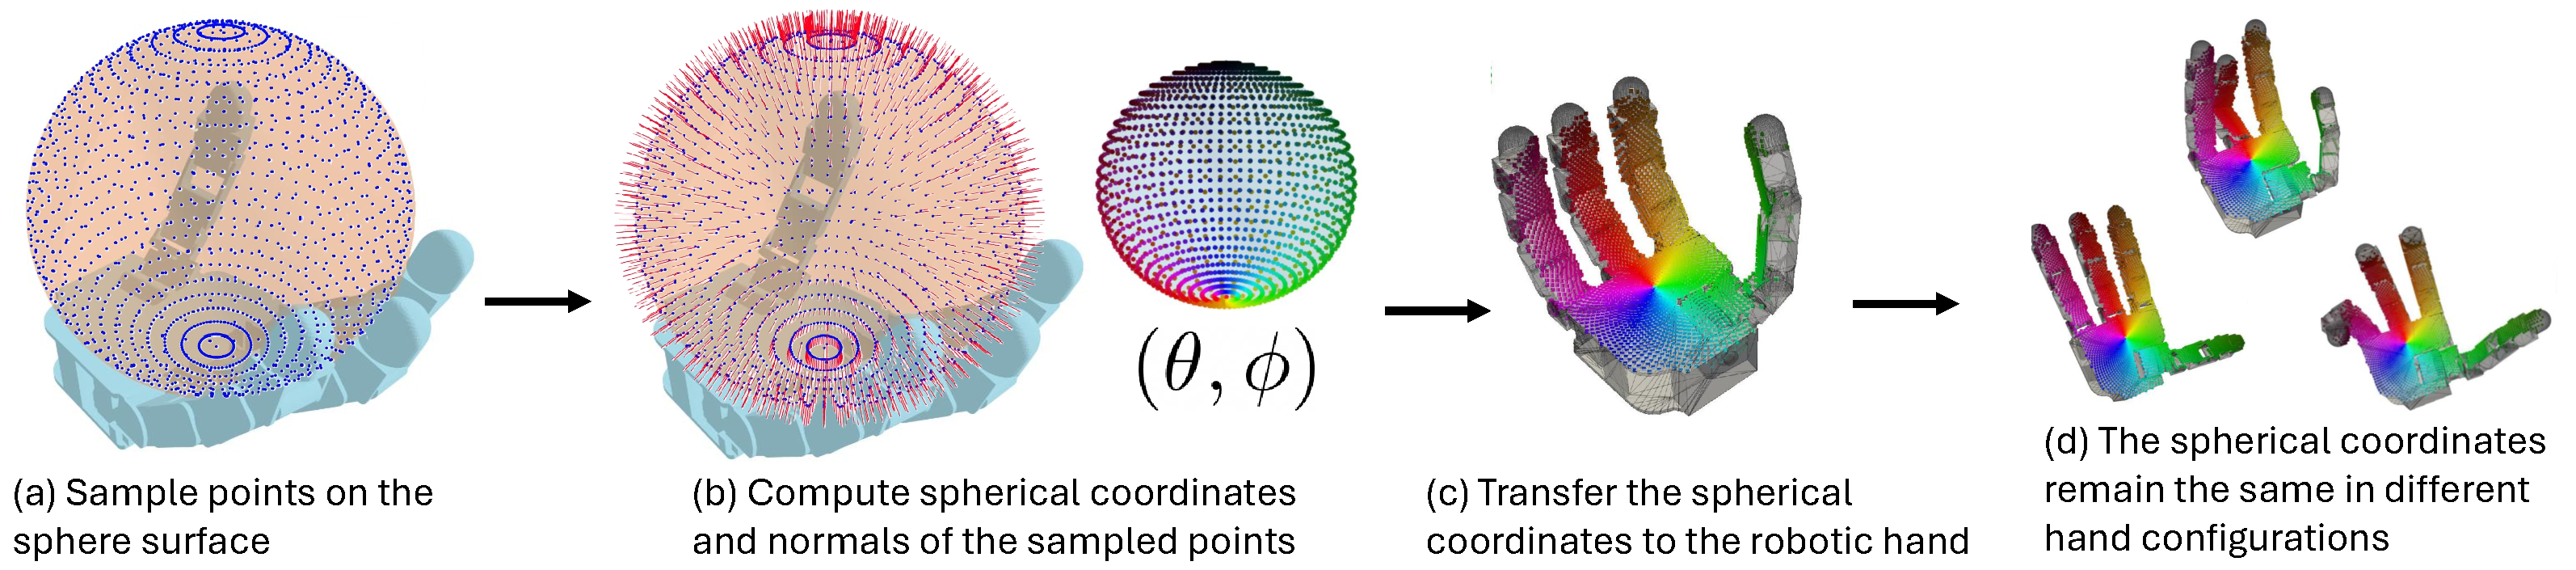
\includegraphics[width=\linewidth]{figures/sphere_correspondence.pdf}
        \caption{Construction of the unified hand surface correspondence.}
    \label{fig:surface_correspondence}
    \end{center}
    \vspace{-6mm}
\end{figure}


\subsection{Unified Hand Surface Correspondence}
\label{sec:surface_correspondence}

The key idea behind using the sphere for hand control is to establish dense geometric correspondences between the canonical sphere surface and the robotic hand. Once these correspondences are defined, deformations of the sphere can be directly transferred to the hand surface, enabling the sphere to serve as a unified action representation across embodiments.

As illustrated in Fig.~\ref{fig:surface_correspondence}, we first uniformly sample points on the sphere surface, as shown in Fig.~\ref{fig:surface_correspondence}(a). For each sampled point, we compute its spherical coordinates $(\theta,\phi)$ together with its outward surface normal, as illustrated in Fig.~\ref{fig:surface_correspondence}(b), where $\theta$ denotes the azimuthal angle and $\phi$ denotes the polar angle. These spherical coordinates provide a canonical parameterization of the sphere surface independent of any specific robotic hand embodiment. We transfer the spherical coordinates to the robotic hand by projecting sampled sphere points onto nearby points on the interior hand surface, producing dense correspondences between the sphere and the palm and finger surfaces, as illustrated in Fig.~\ref{fig:surface_correspondence}(c). Although the 3D locations of the hand surface points vary under different hand configurations, their associated spherical coordinates remain unchanged, as shown in Fig.~\ref{fig:surface_correspondence}(d). This configuration-invariant parameterization enables different robotic hands to share a common spherical coordinate domain, allowing hand actions to be expressed as geometric deformations of the canonical sphere surface rather than embodiment-specific joint motions.



\subsection{Sphere Deformation Action Space}
\label{sec:sphere_deform}

Directly modeling point-wise deformations of the entire sphere surface is computationally impractical due to the high dimensionality of the resulting action space. Let $(\theta,\phi,r)$ denote the spherical coordinates of a point on the normalized reference sphere, where $\theta$ is the azimuthal angle, $\phi$ is the polar angle, and $r=1$ for the undeformed sphere. To obtain a compact action representation, we model sphere deformations using only $(\Delta\theta,\Delta r)$, corresponding to lateral angular displacements and radial expansions or contractions. This simplification is motivated by the construction of the UHAS, where the north pole of the sphere is rigidly anchored to the palm frame.

%Directly modeling deformations of the entire sphere surface on a point-by-point basis is computationally impractical due to the high dimensionality of the resulting action space. Let $(\theta,\phi,r)$ denote the spherical coordinates of a point on the reference (undeformed) sphere, where $\theta$ is the azimuthal angle, $\phi$ is the polar angle, $r$ is the radial coordinate, and $r=1$ for the undeformed sphere after the radius normalization. In the most general case, a sphere deformation can be represented as perturbations $(\Delta\theta,\Delta\phi,\Delta r)$ applied to every surface point.

%To obtain a compact and tractable action representation, we simplify the deformation model to the pair $(\Delta\theta,\Delta r)$. This simplification is motivated by the construction of the Unified Hand Action Space (UHAS), where the north pole of the sphere is rigidly anchored to the palm frame. As a result, the dominant controllable deformations correspond to lateral angular displacements around the sphere and radial expansions or contractions away from the sphere center.

\begin{figure}[h]
 \centering 
 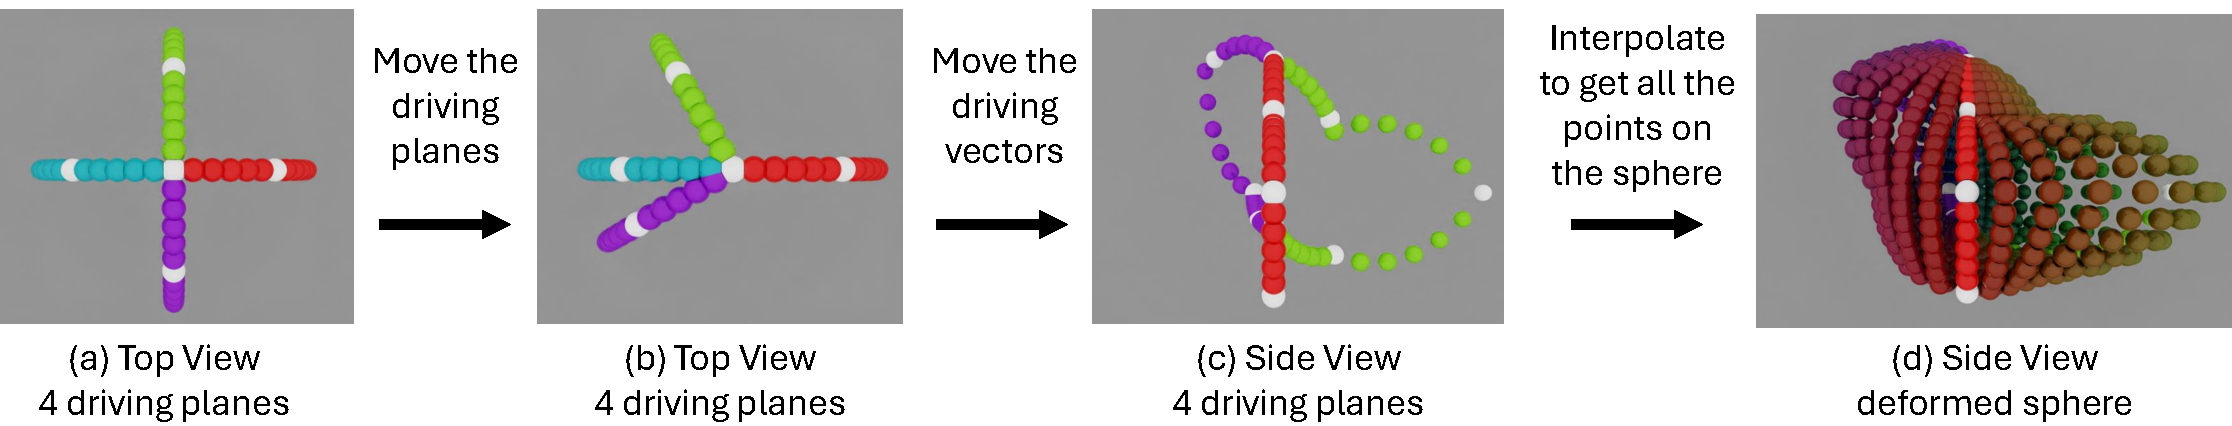
\includegraphics[width=\textwidth ]{figures/sphere_deformation.pdf}\vspace{-2mm}
   \caption{Sphere deformation parameterization in the Unified Hand Action Space (UHAS). 
(a) Initial configuration of four driving planes. 
(b) Rotating the driving planes controls the lateral deformation $\Delta\theta$. 
(c) Radial displacement of the driving vectors controls $\Delta r$. 
(d) The final deformed sphere reconstructed through interpolation.}
   \label{fig:sphere_deformations}
   \vspace{-2mm}
\end{figure}

We parameterize the sphere deformation using a sparse set of \emph{control primitives}. Specifically, we introduce a finite number of \emph{driving planes}, each defined as a plane passing through the sphere center at a fixed azimuthal angle $\theta_{\text{plane}}$ (Fig.~\ref{fig:sphere_deformations}). These driving planes control the lateral deformation component $\Delta\theta$. Within each driving plane, we further define a discrete set of control points at fixed polar angles $\phi$. The radial displacements of these control points, referred to as \emph{driving vectors}, parameterize the radial deformation component $\Delta r$.

The complete deformation field over the sphere surface is reconstructed through interpolation. First, the $\Delta\theta$ deformation at every surface point is obtained by interpolating the values specified by neighboring driving planes. Next, the $\Delta r$ deformation is computed through a two-dimensional interpolation of the driving-vector displacements in the $(\theta,\phi)$ parameter space. Despite the compact parameterization, this representation can generate a rich set of sphere morphologies suitable for dexterous manipulation. Fig.~\ref{fig:sphere_deformations} illustrates an example of a sphere deformation. \emph{If we use five driving planes with two driving vectors per plane, it results in a 15-dimensional continuous action representation, i.e., $5 + 2 \times 5$.} In practice, we define the driving planes such that they align with the hand fingers.


% \subsection{Sphere Deformations}
% \label{sec:sphere_deform}

% Modeling deformations of the entire sphere surface point-by-point is computationally infeasible due to the high dimensionality of the problem. Let $  (\theta, \phi, r)  $ denote the spherical coordinates of any point on the surface of the reference (undeformed) sphere, where $  \theta  $ is the azimuthal angle, $  \phi  $ is the polar angle, and $  r  $ is the radial coordinate. Any deformation of a point can then be expressed as deviations from these reference values, i.e., $  (\Delta\theta, \Delta\phi, \Delta r)  $.

% We simplify the deformation representation to the pair $  (\Delta\theta, \Delta r)  $. This reduction is valid because the north pole of the sphere is rigidly fixed to the gripper palm (by construction of the UGAS section \ref{sec:construction}).

% To control these deformations with a compact set of parameters, we introduce a finite number of ``driving plane'', each defined by a fixed azimuthal angle \(\theta = \theta_{\text{plane}}\). These planes capture the \(\Delta\theta\) component of the deformation. Within each driving plane we further select a discrete set of points at fixed polar angles \(\phi\); we refer to the radial displacements of these points as ``driving vectors'' and use them to encode the $  \Delta r  $ component.

% The full deformation field over the sphere surface is then recovered via linear interpolation. First, the $  \Delta\theta  $ value at every surface point is obtained by interpolating the prescribed deformations from the driving planes. Next, the $  \Delta r  $ value at each point is computed by performing a 2D interpolation over the driving-vector displacements (in the $  \theta  $-$  \phi  $ parameter space). By employing multiple driving planes, each containing several driving vectors, complex sphere morphologies can be realized. The example shown in Fig.~\ref{fig:sphere_deformations} uses five driving planes, each equipped with three driving vectors, for a total of 15 control parameters.

% \begin{figure}[h]
% \centering
% \includegraphics[width=1.0\linewidth]{figures/Fingerclassificationv3.pdf}
% % \caption{Joint classification based on their dominant effect on the fingertip pose in spherical coordinates. The left sequence illustrates encompassing joints, whose motion primarily affects the radial distance $  r  $ or polar angle $  \phi  $, allowing the finger to conform to the sphere surface. The right sequence shows lateral joints, whose motion predominantly changes the azimuthal angle $  \theta  $, enabling side-to-side movement while maintaining contact with the sphere.}
% \caption{Joint classification. Encompassing joints (left) primarily influence the radial distance $  r  $ or polar angle $  \phi  $ to conform the finger to the spherical surface. Lateral joints (right) mainly control the azimuthal angle $  \theta  $, producing lateral movements of the fingertip}
% \label{fig:joint_classification}
% \end{figure}


\subsection{Cascade Inverse Kinematics}
\label{subsec:CIK}

\begin{figure}[h]
    \centering
    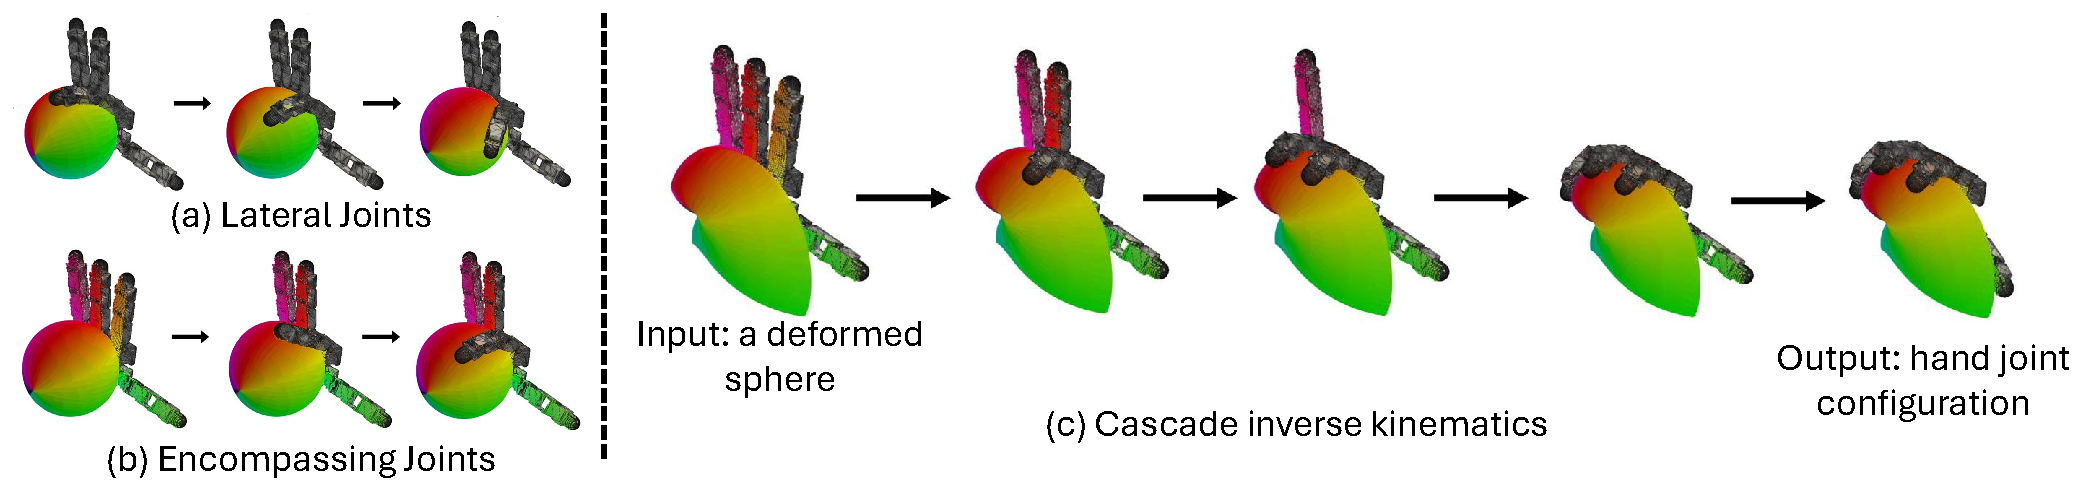
\includegraphics[width=\linewidth]{figures/CIK_new_2.pdf}
    \vspace{-2mm}
    \caption{We classify hand joints into (a) lateral joints and (b) encompassing joints and; (c) Illustration of the cascade inverse kinematics algorithm on a deformed sphere.}
    \label{fig:CIK}
    \vspace{-2mm}
\end{figure}



We map deformed sphere surfaces to embodiment-specific hand joint configurations using a novel \emph{Cascade Inverse Kinematics} (CIK) algorithm. Using the surface correspondences defined in Section~\ref{sec:surface_correspondence}, each hand surface point is associated with fixed spherical coordinates $(\theta,\phi)$ on the canonical sphere. Given a deformed sphere, the corresponding target surface positions are obtained directly from the sphere geometry and used by the CIK algorithm to compute the hand joint configuration $\mathbf{q}$.

\vspace{-2mm}
\paragraph{Joint Classification.}
Each hand joint is classified according to its dominant effect on the corresponding hand surface points in the sphere coordinate frame. As illustrated in Fig.~\ref{fig:CIK}(a), lateral joints primarily control the azimuthal angle $\theta$ of the fingertip and finger surface points, producing side-to-side finger motion. In contrast, encompassing joints in Fig.~\ref{fig:CIK}(b) mainly affect the radial distance $r$ and polar angle $\phi$, allowing the fingers to conform to the sphere surface. This decomposition enables the inverse kinematics problem to be solved efficiently in a cascaded manner.

\vspace{-2mm}
\paragraph{Lateral Joint Mapping.}
 
To efficiently control lateral deformations, we precompute a lookup table by sweeping each lateral joint across its full range of motion while re-solving the encompassing joints on the undeformed reference sphere. For every sampled lateral-joint configuration, we record the resulting fingertip azimuthal angle $  \theta  $. The lookup table provides a mapping between lateral joint configurations and $  \theta  $ displacements on the sphere surface. During inference, the target $  \Delta\theta  $ deformation is obtained directly from the displacement of the fingertip's corresponding sphere point computed in Section~\ref{sec:surface_correspondence}. The lateral joint adjustments $  \Delta\mathbf{q}_{\text{lateral}}  $ are then recovered through direct lookup in the precomputed table.

\vspace{-2mm}
\paragraph{Encompassing Cascade.}
After the lateral adjustment stage, the encompassing joints are solved sequentially along the kinematic chain from the finger root to the fingertip. For each encompassing joint, we solve a one-dimensional inverse kinematics subproblem that places the downstream hand surface points onto their corresponding locations on the deformed sphere surface. This cascading procedure progressively conforms the finger geometry to the target sphere deformation while maintaining kinematic feasibility. The resulting joint configuration $\mathbf{q}$ is the final output of the CIK algorithm. The complete procedure is illustrated in Fig.~\ref{fig:CIK}(c). More details of the CIK algorithm are present in Appendix~\ref{appendix:CIK}.

\paragraph{Sphere Controller.}
By combining the sphere deformation parameterization with the proposed Cascade Inverse Kinematics (CIK) algorithm, we obtain a \emph{sphere controller} that maps sphere deformations in the UHAS to embodiment-specific hand joint configurations. During policy execution, the learned policy predicts sphere deformation parameters, which are converted into executable hand motions through CIK. Thanks to its lightweight sequential structure, CIK runs at up to \textbf{150 Hz}, enabling real-time control across diverse robotic hands.


% With the sphere size, frame, and deformation model fully defined in the Universal Gripper Action Space (UGAS), we now establish the mapping from any deformed sphere to the corresponding gripper joint configuration $  \mathbf{q}  $.
% We achieve this through a novel \emph{cascade inverse kinematics} (CIK) method that solves the inverse kinematics problem sequentially, exploiting the separation of lateral and radial degrees of freedom induced by the sphere representation. 

% \paragraph{Joint classification.}
% Each joint of a finger is classified according to its dominant effect on the fingertip pose in the sphere coordinate frame.

% \begin{itemize}
%     \item \textbf{Encompassing joints}: Joints whose motion predominantly affects the radial distance $  r  $ or the polar angle $  \phi  $ of the finger surface points. These joints are used solely to ``encompass'' or conform the finger to the sphere surface.
%     \item \textbf{Lateral joints}: Joints whose motion primarily changes the azimuthal angle $  \theta  $ of the fingertip. These joints are responsible for lateral (side-to-side) finger movements and are used exclusively for controlling $  \Delta\theta  $.
% \end{itemize}





% \paragraph{Solving for an input Sphere}


% Starting from the root of each finger and proceeding sequentially to the tip along the kinematic chain, we solve for every encompassing joint as follows: we identify the sphere surface points reachable by the current link length and compute the joint angle that places the link surface directly onto the sphere surface.

% For the lateral joints use a precomputed a lookup table by sweeping each lateral joint over its full range of motion. For every sampled lateral-joint value we re-solve the encompassing joints on a perfect undeformed sphere, then record the resulting $  \theta  $ coordinate of the fingertip. For any deformed sphere the lateral deformations are calculated with respect to a reference positon at the center of their $ \theta $ range. 

% The perfect-sphere configuration $  \mathbf{q}_{G_S}  $ is obtained by setting each lateral joint to the midpoint value of its $  \theta  $ range in the lookup table with the corresponding encompassing joint values.
% During the sweep we apply a polar-angle threshold on the fingertip to guarantee that the encompassing joints remain within a valid workspace and do not point away from the sphere (a precaution especially relevant for grippers with large range of motion such as the Leap Hand~\cite{shaw2023leaphand}). 

% Ensuring the fingerprint points are driven to a nearby feasible position on the deformed surface.

% Given the deformations $  (\Delta\theta, \Delta r)  $ at the driving planes and driving vectors (see Section~\ref{sec:sphere_deform}). The CIK is performed sequentially on every finger as follows: First, a lateral adjustment corresponding to the $  \Delta\theta  $ deformation of the fingertip's corresponding point on the deformed sphere is read directly from the upsampled surface. The required change in the lateral joint angles $  \Delta\mathbf{q}_{\text{lateral}}  $ is obtained by direct lookup in the precomputed table. Second, the kinematic chain is traversed from root to tip. For each encompassing joint we solve a one-dimensional inverse kinematics subproblem that places the reachable surface points of the downstream link onto the deformed sphere. 
% The resulting joint configuration $  \mathbf{q}_t  $ is the final output of the CIK. The procedure is illustrated in Figure~\ref{fig:CIK}.
% , we first reconstruct the full deformed sphere surface by linear interpolat\textbf{}ion and upsampling. 


% \begin{enumerate}
% \item \textbf{Lateral adjustment}: The $  \Delta\theta  $ deformation of the fingertip's corresponding point on the deformed sphere is read directly from the upsampled surface. The required change in the lateral joint angles $  \Delta\mathbf{q}_{\text{lateral}}  $ is obtained by direct lookup in the precomputed table.
% \item \textbf{Encompassing cascade}: The kinematic chain is traversed from root to tip. For each encompassing joint we solve a one-dimensional inverse kinematics subproblem that places the reachable surface points of the downstream link onto the deformed sphere. This process continues until the fingertip is reached.
% \end{enumerate}



% The CIK provides an efficient and general mapping from sphere deformations in the UHAS to realistic joint configurations across a wide variety of robotic grippers. Figure~\ref{fig:multigripper_CIK} demonstrates the CIK applied to multiple robotic hands under identical sphere deformations, underscoring the generalizability of the proposed approach.

% \begin{figure}[h]
%     \centering
%     \includegraphics[width=\linewidth]{figures/Grippers_same_sphere.pdf}
%     \caption{Illustration of the cascade inverse kinematics (CIK) procedure of the same deformed sphere on multiple hands.}
%     \label{fig:multigripper_CIK}
% \end{figure}

